% !TeX root = ../main.tex

\chapter{Introduction}\label{chapter:Introduction}

Ever since the dawn of video games, the focus has been concentrated on making virtual worlds look as realistic as possible. Advances in \gls{cga} techniques as well as continuously increasing processing power have allowed even real time \gls{cga} to become almost photo-realistic \autocite{photorealismRealtime}.
\newline
An example for this evolution in graphical fidelity is the comparison of \textit{id Software}'s \textit{Doom} video games from 1993 and 2016 in \autoref{fig:doom1993vs2016}. The basic way the game is played has stayed essentially the same: buttons on the keyboard trigger actions displayed on the screen, which acts as a window into the virtual world. The largest difference is the drastically more believable presentation of the game world, which is a comparatively easily quantifiable improvement of player \gls{immersiongl} \autocite{gameImmersion}. This thesis, however, will explore a different avenue to increased player \gls{immersiongl}.

\begin{figure}[h]%[!tbp]
  \centering
  \subfloat[Doom1993][Doom 1993 \autocite{gamestarDoomPics}]{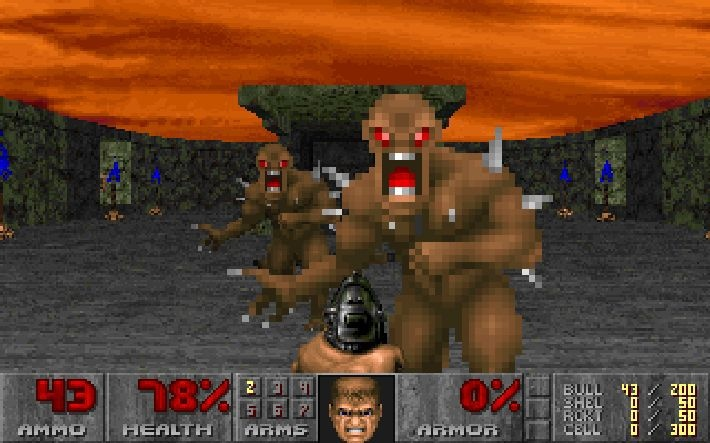
\includegraphics[height=0.2\textheight]{figures/doom1993.jpg}\label{fig:doom1993}}
  \hfill
  \subfloat[Doom2016][Doom 2016 \autocite{newGameNetworkDoomPics}]{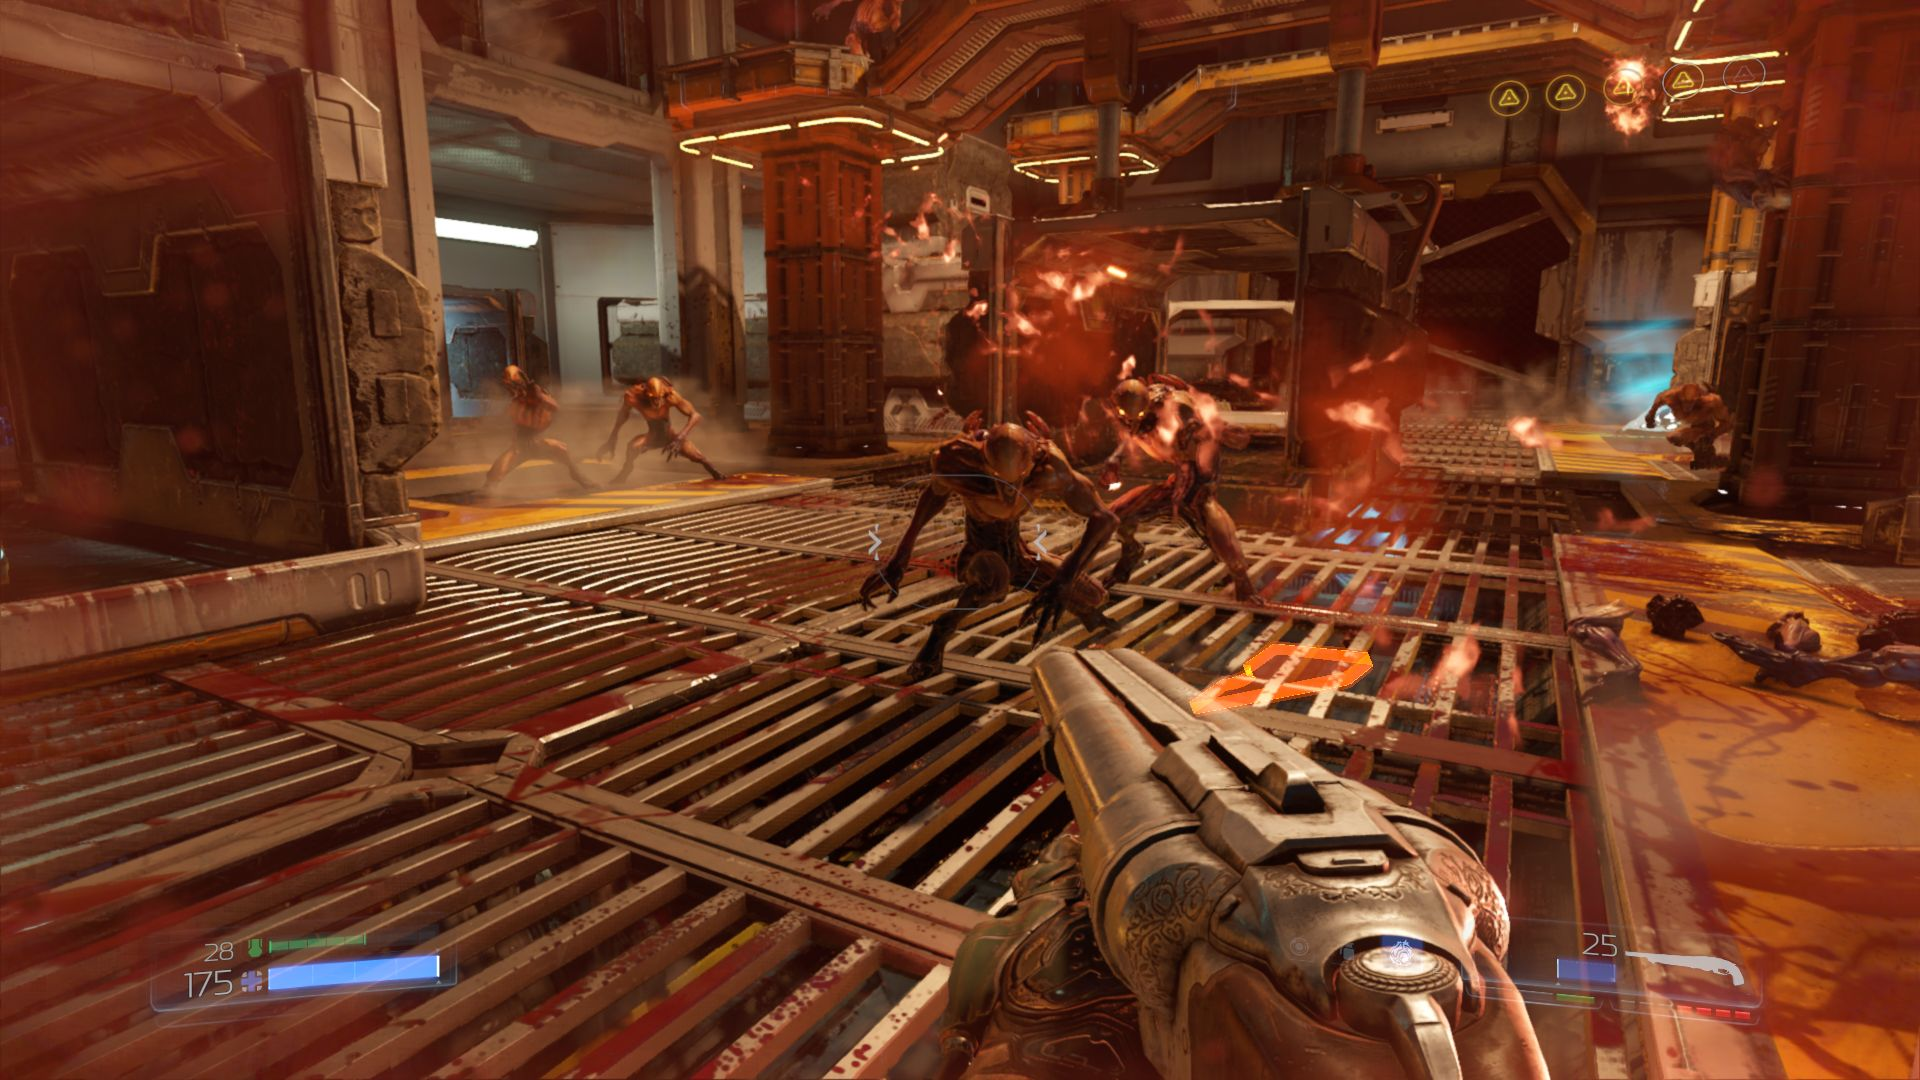
\includegraphics[height=0.2\textheight]{figures/doom2016}\label{fig:doom2016}}
  \caption{Evolution of \gls{cga} exemplified by \textit{Doom} games}
  \label{fig:doom1993vs2016}
\end{figure}

The rise of high quality \gls{vra} has allowed users to not only look into a virtual world, but to see it as if they were actually part of it. There are various factors which influence how effective the illusion of being part of a virtual environment is. This thesis will focus on one: giving the user a fully animated body, as \enquote{a virtual body in the context of a head-mounted display based virtual reality is a critical contributor to the sense of being in the virtual location} \autocite[p.~374]{senseEmbodimentVR}. This is commonly referred to as \textit{virtual embodiment}, of which a more in depth discussion will follow in \autoref{chapter:VirtualEmbodiment}.
\newline

A problem that arises when giving the user a body in \gls{vra} is that the virtual world can influence the virtual body, exerting forces on it, but not on the real body of the user. This can result in situations where the real and virtual body become mismatched due to, for example, the tracked position of a real hand being inside a virtual object, such as a wall, and the virtual hand not following into the object.
\newline
One effect of such discrepancies being handled inadequately, is motion sickness. According to James Lackner, \enquote{The sensory conflict theory of motion sickness proposed by Reason \textelp{} is the most widely accepted theory of motion sickness} \autocite[p. ~11]{motionSickness}.Here it is stated that a discrepancy between visually perceived motion and bodily felt motion, is the main cause of motion sickness.
\newline
Another problem that arises when such discrepancies are ignored, is that the user can, for example, stick his head through a wall, and is thus able to see parts of the environment he should normally not be able to, or even to walk through obstacles to interact with objects he is not meant to be able to access. From the environment designer's point of view, this is problematic since the designer is not in full control of where the player can be at all times. From the user's perspective, these abilities, depending on the context, can impair his \gls{immersiongl}, since he is able to do impossible things.
\newline
Assuming, that the user's virtual limbs will not follow his tracked, real limbs into (in the virtual world) impossible states, one could assume that it would be simple for the user to correct his pose. However the Rubber Hand Illusion experiment\footnote{In experiments, stimulating a test subject's hidden hand as well as a rubber hand placed in view before them simultaneously in the same manner, caused the test subject to mislocate his real, hidden hand.} shows that the human body is not adept at locating unseen parts of itself \autocite{rubberHandsFeel}, so we cannot rely on the user's sense of \gls{kinesthesiagl} to tell him where his real body parts are.
\newline

In an effort to mitigate these problems, methods for alerting the user to discrepancies between his real and his virtual body which will allow him to easily adjust his pose to match that of his virtual body, especially with respect to his feet, will be investigated. 

